\begin{frame}
\frametitle{Aircraft W\&B}
\begin{center}
Fixed-wing Aircraft Weight and Balance
\end{center}
\end{frame}

\begin{frame}
\frametitle{Fixed-wing Aircraft Weight and Balance}
\begin{block}{Basic principles}
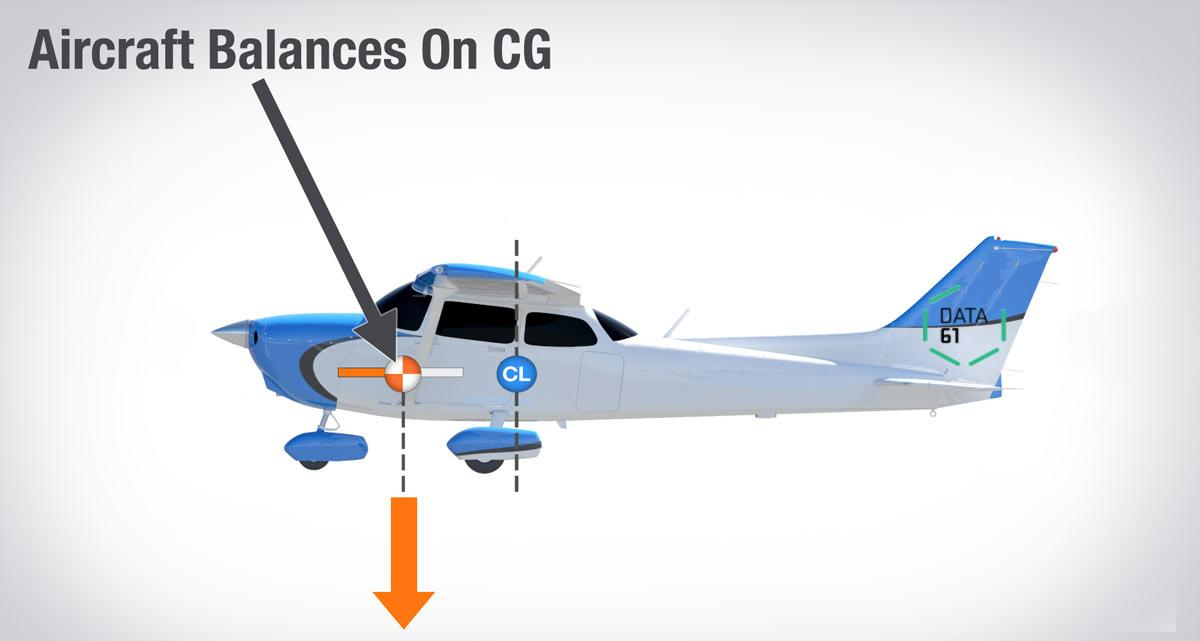
\includegraphics[height=0.5\textheight]{image/aircraft-cg.jpg}
\end{block}
\end{frame}

\begin{frame}
\frametitle{Fixed-wing Aircraft Weight and Balance}
\begin{block}{Same principles apply to A380}
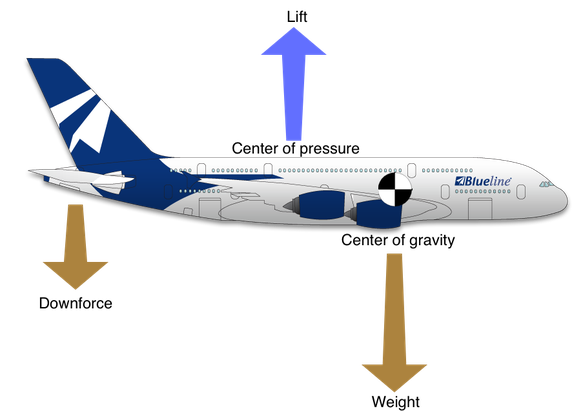
\includegraphics[height=0.5\textheight]{image/aircraft-cg-a380.png}
\end{block}
\end{frame}

\begin{frame}
\frametitle{Fixed-wing Aircraft Weight and Balance}
\begin{block}{Weight, Balance \emph{\tiny{loosely speaking}}}
\begin{itemize}
\item Weight is ensuring that the aircraft is not too heavy to maintain flight.
\item Balance is ensuring that the CG is positioned such that the aircraft is controllable.
\end{itemize}
\end{block}
\end{frame}

\begin{frame}
\frametitle{Fixed-wing Aircraft Weight and Balance}
\begin{block}{This is a Cessna 172S}
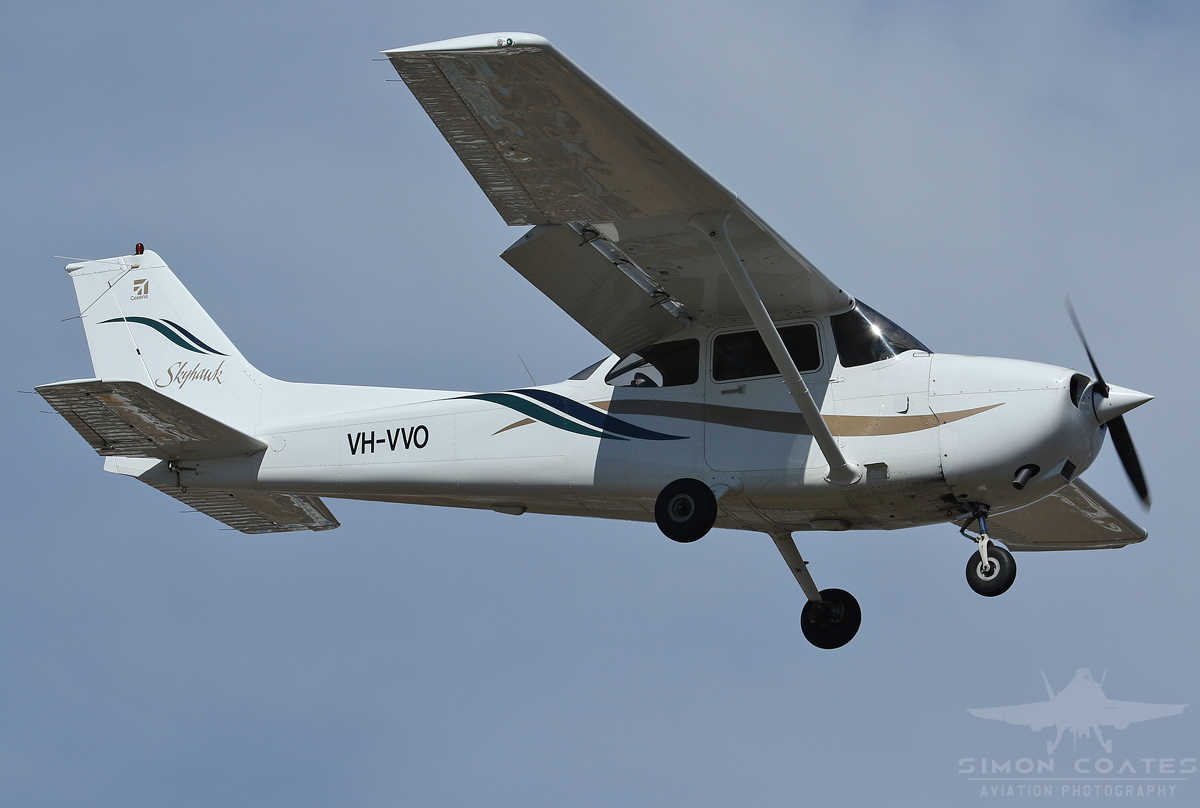
\includegraphics[height=0.5\textheight]{image/vhvvo.jpg}
\end{block}
\end{frame}

\begin{frame}
\frametitle{Fixed-wing Aircraft Weight and Balance}
\begin{block}{Cessna 172S}
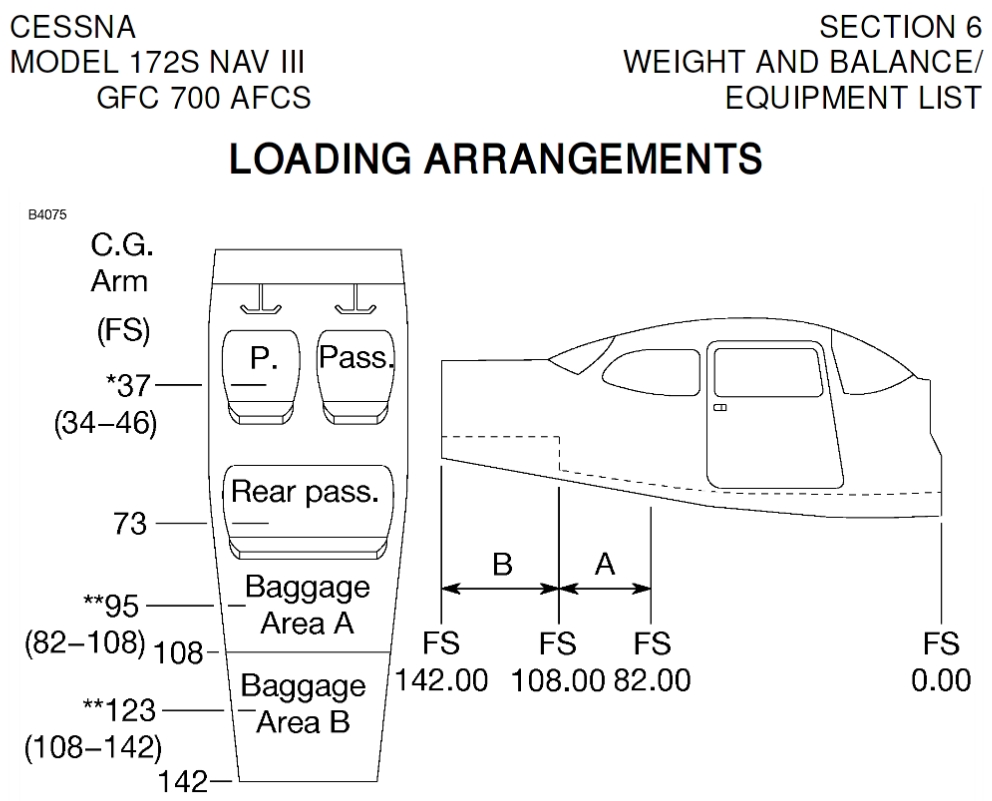
\includegraphics[height=0.5\textheight]{image/c172-loading.png}
\begin{itemize}
\item 2x2 seating arrangement
\item 2 baggage areas
\end{itemize}
\end{block}
\end{frame}

\begin{frame}
\frametitle{Fixed-wing Aircraft Weight and Balance}
\begin{block}{VH-VVO}
Let's go flying!
\end{block}
\end{frame}

\begin{frame}
\frametitle{Fixed-wing Aircraft Weight and Balance}
\begin{block}{VH-VVO}
but first, let's do a weight and balance :)
\end{block}
\end{frame}

\begin{frame}
\frametitle{Fixed-wing Aircraft Weight and Balance}
\begin{block}{VH-VVO}
\begin{itemize}
\item \tiny{\emph{page 190 PoH LOADING GRAPH}}
\item \tiny{\emph{page 194 PoH CG Moment Envelope}}
\item \tiny{VH-VVO}
  \begin{itemize}
  \item \tiny{BEW 1684.3 pounds}
  \item \tiny{CG arm 40.6 inches}
  \end{itemize}
\end{itemize}
\end{block}
\end{frame}

\begin{frame}
\frametitle{Fixed-wing Aircraft Weight and Balance}
\begin{block}{VH-VVO}
\begin{itemize}
\item \tiny{\emph{Consider also TODR/LDR}}
  \begin{itemize}
  \item \tiny{linearly interpolate weight}
  \item \tiny{linearly interpolate pressure altitude}
  \item \tiny{linearly interpolate temperature}
  \end{itemize}
\end{itemize}
\end{block}
\end{frame}

\begin{frame}
\frametitle{Fixed-wing Aircraft Weight and Balance}
\begin{block}{VH-VVO}
\begin{itemize}
\item<1-> I typically perform W\&B 24 hours prior to flight.
\item<2-> Assuming I can obtain the specific aircraft BEW and CG arm.
\item<3-> Then double-check, then verbalise it to myself, then check again.
\item<4-> With no time pressure or other distractions.
\end{itemize}
\end{block}
\end{frame}

\begin{frame}
\frametitle{Fixed-wing Aircraft Weight and Balance}
\begin{block}{then this happens}
\begin{itemize}
\item<1-> Operator: ``We've changed your aircraft to VH-LSE.''
\item<2-> New BEW, CG arm or fuel quantity.
\item<3-> Jessica: ``Hey is it cool if I sit in the front?''
\item<4-> I now have time pressure and distractions.
\item<5-> I am tempted to use my previous calculations and declare the difference insignificant.
\end{itemize}
\end{block}
\end{frame}

\begin{frame}
\frametitle{Fixed-wing Aircraft Weight and Balance}
\begin{block}{Pass arguments to functions}
\begin{itemize}
\item<1-> This W\&B calculation is \textbf{just a function} to which we are applying \textbf{arguments}.
\item<2-> I wonder if we have good tools for doing this already?
\item<3-> You know, writing functions
\item<4-> and passing arguments to them
\end{itemize}
\end{block}
\end{frame}

\begin{frame}
\frametitle{Fixed-wing Aircraft Weight and Balance}
\begin{center}
Let's write the code.
\end{center}
\end{frame}

% being under time pressure when a variable changes
